\documentclass[11pt, onecolumn]{article}
\usepackage[margin=2.5cm]{geometry}
\usepackage[T1]{fontenc}
\usepackage{lmodern}
\usepackage[protrusion=true,expansion=true,final]{microtype}
\usepackage[hidelinks]{hyperref}
\usepackage[style=vancouver, backend=biber]{biblatex}
\usepackage{booktabs}
\usepackage{caption}
\usepackage{subcaption}
\usepackage{graphicx}
\usepackage{xcolor}
\usepackage{amsmath}
\usepackage{algorithm}
\usepackage{algpseudocode}
\usepackage{tikz}
\usetikzlibrary{positioning,arrows.meta}
\captionsetup{font=small, labelfont=bf}
\setlength{\parindent}{0pt}
\setlength{\parskip}{6pt}

% Placeholder command for missing numbers/figures in draft
\newcommand{\placeholder}[1]{\textcolor{red}{\textbf{[#1]}}}

\addbibresource{references.bib}

\title{kam: Alignment-Free Variant Detection for Duplex UMI Sequencing\\
\large v0.2}
\author{Trent Zeng}
\date{March 2026}

\begin{document}
\maketitle

\begin{abstract}
Detecting somatic variants at sub-1\% allele frequency in liquid biopsy samples
requires accurate UMI-based error suppression and sensitive variant calling.
Current pipelines chain several tools that discard molecule-level information
between steps, making per-molecule strand bias and duplex evidence unavailable
at the calling stage.

We present kam, an alignment-free variant detection pipeline for Twist duplex
UMI panel sequencing. kam assembles duplex molecules directly from raw FASTQ,
indexes k-mers with per-molecule provenance, builds a de Bruijn graph over all
observed k-mers, and calls variants by scoring alternative paths against the
reference path using molecule counts and strand composition. No reference
alignment is performed. Called variants are left-normalised to standard VCF
convention, enabling direct comparison against truth sets for SNVs, indels, and
structural variants. Structural variant detection uses junction k-mer injection:
breakpoint-spanning k-mers are added to the allowlist, making SV allele paths
discoverable in the de Bruijn graph without specialised alignment.

We evaluate kam in two operating modes on the Twist cfDNA Pan-Cancer Reference
Standard v2 titration series (375 truth variants, 24 samples, 5--30\,ng input
DNA, VAF 0\%--2\%). In discovery mode, kam detects 54--63\% of truth variants
at 2\% VAF with precision 0.69--0.84 using 2M read pairs per sample. In
tumour-informed monitoring mode (\texttt{--target-variants}), the same calls
are filtered to variants matching a pre-specified target VCF: precision rises
to 1.0 at all VAF levels with no change to sensitivity.

We identified and fixed two implementation bugs during evaluation: a strand
bias overcounting bug that inflated the Fisher exact test sample size
approximately 70-fold, and a duplex orientation comparison bug that prevented
genuine duplex pairs from being grouped correctly.
With both fixes applied and 2M read pairs per sample, duplex identification
rates are 6.2--18.9\% of molecules. With recommended filters
(\texttt{--max-vaf 0.35 --min-family-size 2}) and tumour-informed mode applied,
kam detects 54--63\% of truth variants at 2\% VAF with precision 1.0, running
end-to-end in 41--55 seconds per sample on a single core. SNV sensitivity
reaches 69--80\% at 2\% VAF; indel sensitivity is 32--39\%. Sensitivity at
0.25--0.5\% VAF reaches 26--46\% at 15--30\,ng input and 6--17\% at 5\,ng input.

kam is implemented in Rust and is available as an open-source workspace.

\end{abstract}

\section{Introduction}
\label{sec:introduction}

Circulating tumour DNA (ctDNA) in blood plasma carries somatic variants shed from solid tumours.
Detecting these variants enables non-invasive cancer monitoring: tracking treatment response, identifying resistance mutations, and detecting minimal residual disease\autocite{Wan17ctdna}.
The challenge is sensitivity.
Clinically relevant ctDNA fractions range from 2\% down to 0.001\% of total cell-free DNA, depending on tumour burden and stage.
At these variant allele frequencies (VAFs), a single mutant molecule must be distinguished from thousands of wild-type molecules and from sequencing errors that occur at rates of $10^{-2}$ to $10^{-3}$ per base.
Duplex UMI sequencing suppresses these errors by tagging each original DNA molecule with a unique molecular identifier (UMI) before amplification, then requiring that both strands of the molecule independently confirm each base call\autocite{Schmitt12duplex, Kennedy14duplex}.
This reduces the effective error rate to approximately $10^{-7}$ per base, making sub-0.1\% VAF detection possible in principle.

Alignment-free variant detection using k-mer counting and de Bruijn graph path walking was established as a viable alternative to alignment-based calling for UMI duplex data.
The standard pipeline chains HUMID for UMI-based deduplication\autocite{Langedijk22humid}, Jellyfish for k-mer counting\autocite{Marcais11jellyfish}, km for de Bruijn graph path walking\autocite{Bourgey19km}, and kmtools for parallelisation and filtering.
This pipeline discards molecule identity at the first step.
HUMID collapses read families into single representative reads.
Jellyfish then counts k-mers across all surviving reads, producing a hash table of integer counts with no record of which molecules contributed each count.
km walks paths through the resulting de Bruijn graph and calls variants using a ratio threshold on these aggregate counts.
The duplex strand information, the per-molecule error correction, and the family size metadata are all lost before variant calling begins.

This information loss has two consequences.
First, variant evidence is inflated by PCR duplicates, increasing false positive rates at low VAF.
Second, the variant caller cannot distinguish high-confidence duplex-confirmed variants from low-confidence simplex singletons.
Both look the same in a table of integer k-mer counts.

We present kam, a single Rust tool that replaces the full four-tool pipeline and preserves molecule provenance from raw FASTQ reads through to variant calls.
kam extracts UMIs directly from FASTQ reads, groups reads into duplex molecule families, builds consensus sequences with quality-weighted error correction, and indexes k-mers with per-k-mer \texttt{MoleculeEvidence}: the number of distinct molecules, the number with duplex support, the strand breakdown, and per-base error probabilities.
Variant calling operates on molecule counts, not read counts, and uses a statistical model that weights duplex-confirmed evidence above simplex evidence.

kam supports two operating modes.
In \emph{discovery mode}, it finds all alternative paths within each 100\,bp target window and reports every path that passes statistical quality filters.
In \emph{tumour-informed mode} (\texttt{--target-variants}), a VCF of expected somatic variants is provided and the caller only reports calls whose (CHROM, POS, REF, ALT) matches an entry in that set.
Discovery mode is appropriate for initial somatic profiling; tumour-informed mode is appropriate for serial liquid biopsy where the variant panel is known from a prior biopsy.

On the Twist cfDNA Pan-Cancer Reference Standard v2 titration series with tumour-informed filtering applied, kam detects 52--61\% of truth variants at 2\% VAF with precision 1.0 (zero false positives), running in 19--35 seconds per sample on a single core.

Section~\ref{sec:background} covers duplex UMI sequencing and k-mer variant detection.
Section~\ref{sec:related_work} reviews existing tools and their limitations.
Section~\ref{sec:method} describes kam's architecture, from molecule assembly through statistical calling.
Sections~\ref{sec:results} and~\ref{sec:evaluation} present benchmark results on the titration dataset.

\section{Background}
\label{sec:background}

\subsection{Duplex UMI sequencing}
\label{sec:bg-duplex}

Standard next-generation sequencing produces per-base error rates of $10^{-2}$ to $10^{-3}$, set by the accuracy of the sequencing chemistry.
Detecting a variant at 0.1\% VAF requires distinguishing a true signal from errors that occur at 10 to 100 times the signal frequency.
Duplex UMI sequencing solves this through two layers of error correction\autocite{Schmitt12duplex}.

Before PCR amplification, each original DNA molecule receives a pair of UMI tags, one ligated to each strand.
All PCR copies of that molecule carry the same UMI pair.
After sequencing, reads sharing a UMI pair are grouped into a \emph{molecule family}.
The first error correction step collapses all reads from one strand of a family into a \emph{single-strand consensus sequence} (SSC) by majority vote weighted by base quality.
Positions where most reads agree are called with high confidence; positions where reads disagree are flagged or masked.
This reduces the error rate to approximately $10^{-3}$ to $10^{-4}$, limited by systematic errors that affect all copies of one strand identically.

The second step compares the forward-strand SSC to the reverse-strand SSC.
A sequencing or PCR error on one strand is unlikely to produce the identical error on the complementary strand independently.
Positions where both SSCs agree form the \emph{duplex consensus sequence} (DCS), with an effective error rate of approximately $10^{-7}$: the product of the two independent per-strand error rates\autocite{Kennedy14duplex}.
This three-order-of-magnitude improvement over single-strand consensus is what makes sub-0.1\% VAF detection feasible.

The Twist Biosciences UMI adapter system\autocite{Twist22cfdna} uses the read structure \texttt{5M2S+T} on both R1 and R2: 5 bases of random UMI, 2 bases of skip sequence (a fixed monotemplate spacer from the ligation chemistry), and the remaining template sequence.
The 5-base UMI provides $4^5 = 1{,}024$ possible UMI values.
Duplex strand pairing uses a canonical form: given UMI pair $(A, B)$ from R1 and R2, the canonical identifier is $\min(A{+}B,\; B{+}A)$ by lexicographic order.
Reads with UMI pair $(A, B)$ and reads with UMI pair $(B, A)$ map to the same molecule on opposite strands.

The small UMI space creates a collision problem at high sequencing depth.
At 10{,}000$\times$ coverage, two unrelated molecules at the same genomic locus can share a UMI pair by chance.
Collisions merge distinct molecules into one family, masking real variants (false negatives) or averaging unrelated sequences (consensus errors).
Collision detection requires a secondary signal beyond the UMI itself, such as the genomic endpoints of the sequenced fragment.

\subsection{K-mer approaches to variant detection}
\label{sec:bg-kmer}

A k-mer is a subsequence of length $k$ extracted from a read or reference.
For $k = 31$, a 150-base read yields 120 overlapping 31-mers.
K-mer counting tools such as Jellyfish\autocite{Marcais11jellyfish} build a hash table mapping each distinct k-mer to its occurrence count across all input reads.
This index supports alignment-free analyses: any query about sequence content can be answered by looking up k-mer counts without aligning reads to a reference genome.

K-mer variant detection works by constructing a de Bruijn graph from the k-mer index and walking paths through it.
Each node in the graph is a k-mer; edges connect k-mers that overlap by $k{-}1$ bases.
Given a target reference sequence (for example, exon 7 of \emph{TP53}), the tool anchors the walk at the first and last k-mers of the reference, then enumerates all paths between these anchors that are supported by k-mer evidence in the index.
The reference path represents the wild-type allele.
Any alternative path represents a variant: a single-nucleotide substitution adds one divergent node, an insertion adds extra nodes, and a deletion skips nodes.
The ratio of variant-path k-mer counts to reference-path k-mer counts estimates the VAF.

km\autocite{Bourgey19km} implements this approach using Jellyfish k-mer databases.
It was designed for RNA-seq mutation detection and calls variants when the count ratio exceeds a user-specified threshold (the \texttt{-{}-ratio} parameter).
This threshold is a global cutoff with no statistical model: the same ratio at 100$\times$ and 10{,}000$\times$ coverage receives the same call, despite representing very different levels of evidence.
kmtools adds parallelisation (chunking targets across processes) and post-hoc filtering against known variant databases.

The fundamental limitation of this pipeline is that k-mer counts are integers with no provenance.
Jellyfish's canonical mode (\texttt{-C}) collapses forward and reverse-complement k-mers into a single count, erasing strand information entirely.
There is no per-k-mer record of how many molecules contributed the count, whether those molecules had duplex support, or what the base qualities were at the variant position.

\subsection{The information loss problem}
\label{sec:bg-information-loss}

The existing pipeline processes data through four stages, losing information at each transition.
Figure~\ref{fig:info-loss} illustrates the two pipelines side by side.

\begin{figure}[htbp]
\centering
\small
\begin{verbatim}
Existing pipeline:
  Raw reads --> HUMID (dedup) --> Jellyfish (count) --> km (call)
  [duplex       [one read        [integer              [ratio
   families,     per family,      counts,               threshold,
   strand info,  no consensus,    no strand,            no statistics,
   base quality] no metadata]     no molecules]         no confidence]

kam pipeline:
  Raw reads --> molecule assembly --> k-mer index --> variant calling
  [duplex       [SSC + DCS           [MoleculeEvidence  [molecule-count
   families,     consensus,           per k-mer:          statistics,
   strand info,  quality scores,      n_molecules,        duplex-aware
   base quality] family metadata]     n_duplex,           weighting,
                                      strand counts,      confidence
                                      error probs]        intervals]
\end{verbatim}
\caption{Information flow in the existing pipeline (top) and kam (bottom).
Each arrow represents a processing step.
Brackets list the information available at that stage.
The existing pipeline reduces duplex molecule families to integer k-mer counts by the second step.
kam preserves molecule identity and quality metadata through to variant calling.}
\label{fig:info-loss}
\end{figure}

Three specific losses matter for low-VAF variant detection.

\textbf{Loss of molecule identity.}
HUMID selects one representative read per UMI group and discards the rest.
Jellyfish then counts k-mers across all surviving reads.
A k-mer count of 500 could represent 500 independent molecules (strong evidence) or 5 molecules with 100 PCR copies each (weak evidence).
The distinction is critical at 0.1\% VAF, where a true variant may be supported by only 5 to 10 molecules out of 5{,}000 to 10{,}000 total.

\textbf{Loss of strand information.}
Jellyfish's canonical k-mer mode merges forward and reverse-complement k-mers.
A variant supported by molecules on only one strand is a hallmark of systematic artefact (oxidative damage, deamination), not a true somatic mutation.
Without strand information, the variant caller cannot apply strand bias filters.

\textbf{Loss of error correction quality.}
Duplex consensus bases have error rates of ${\sim}10^{-7}$.
Simplex consensus bases have error rates of ${\sim}10^{-3}$.
Singleton reads have error rates of ${\sim}10^{-2}$.
When all are collapsed into a single k-mer count, the variant caller treats evidence from a duplex-confirmed molecule identically to evidence from an uncorrected singleton.
A principled statistical model should weight these differently.

kam addresses all three losses by storing \texttt{MoleculeEvidence} per k-mer: distinct molecule count, duplex molecule count, per-strand simplex counts, and aggregate error probabilities.
The variant caller uses these fields directly, calling variants based on the number of independent molecules (not reads) and weighting duplex evidence above simplex evidence.

\section{Related Work}
\label{sec:related_work}

\subsection{UMI Deduplication Tools}

UMI deduplication tools group raw reads by UMI identity and produce a single consensus read per molecule group. UMI-tools \autocite{Smith17umitools} introduced network-based grouping methods (directional, adjacency, and cluster) where nodes represent UMIs and edges connect UMIs within a fixed edit distance. This corrects for sequencing errors in the UMI itself and remains the most widely cited method in the literature. HUMID \autocite{Langedijk22humid} takes a reference-free approach, using a trie over UMI sequences to perform Hamming-distance grouping directly on FASTQ input without prior alignment. fgbio \autocite{fgbio} is the de facto clinical standard for duplex UMI workflows: its \texttt{GroupReadsByUmi} and \texttt{CallDuplexConsensusReads} stages produce a single-strand consensus per strand and a duplex consensus where both strands agree. UMICollapse \autocite{Liu19umicollapse} achieves order-of-magnitude speed improvements over UMI-tools using N-gram indexing and BK-trees. Commercial tools such as the Sentieon ctDNA pipeline offer a 2--3$\times$ end-to-end speedup at the cost of being closed source.

All of these tools share a common output model: a deduplicated FASTQ or BAM file where each record represents one consensus read. The molecule identity that produced each consensus, including whether it was duplex or simplex, how many raw reads supported it, and which strand each read came from, is either discarded entirely or encoded in SAM auxiliary tags that downstream tools rarely use. In fgbio's own benchmarks, consensus base quality scores generated by \texttt{CallDuplexConsensusReads} were not propagated into variant calling \autocite{fgbio}, which means the duplex-level confidence information was computed and then ignored.

kam differs from this family by making the molecule the primary unit of analysis throughout the pipeline. Molecule provenance, duplex status, strand family size, and per-base confidence are not metadata appended to a read record; they are first-class fields in the \texttt{MoleculeEvidence} type that flows from assembly through k-mer indexing to variant calling. This propagation is what enables duplex-aware scoring at the calling stage.

\subsection{K-mer-Based Variant Detection}

The km/kmtools pipeline \autocite{Bourgey19km} uses Jellyfish \autocite{Marcais11jellyfish} k-mer counts as the basis for alignment-free variant detection. Jellyfish counts k-mer occurrences in a set of sequences using a lock-free hash table and outputs per-k-mer integer counts. km walks de Bruijn graph paths built from those counts to find sequence variants: it identifies k-mers present in a sample but absent or underrepresented in a reference, then assembles those k-mers into candidate variant sequences. This approach handles insertions, deletions, and SNVs without reference alignment, avoiding alignment bias in repetitive regions. kmtools parallelises km across a target panel and aggregates results.

The core limitation is that Jellyfish stores integer counts only. It has no concept of read origin, molecule identity, or quality. The canonical k-mer flag (\texttt{-C}) collapses both strands into the same counter, erasing strand information entirely. A k-mer count of 10 could represent ten PCR duplicates from a single molecule or ten independent molecules, and Jellyfish cannot distinguish them. Quality scores are ignored, so a k-mer supported by ten Q10 reads looks identical to one supported by ten Q40 reads. km's variant calling uses a global ratio threshold (\texttt{--ratio}) with no statistical model: the same threshold is applied regardless of sequencing depth, which means the false positive rate changes with coverage even when the true VAF is constant.

kam differs from this family by replacing integer k-mer counts with \texttt{MoleculeEvidence}: each k-mer entry records the number of distinct molecules that contributed it, broken down by duplex, simplex-forward, and simplex-reverse. Variant calling operates on molecule counts under a binomial model with a per-site background, not on a global ratio threshold. Duplex molecules, whose error rate is approximately $10^{-7}$ compared to $10^{-2}$ for a single read, receive higher statistical weight. This allows depth-calibrated confidence intervals and strand-bias detection as a first-class filter.

\subsection{Alignment-Based Low-VAF Variant Callers}

The dominant approach to somatic variant detection in ctDNA is to align reads to a reference genome and call variants from the resulting BAM file. GATK Mutect2 \autocite{McKenna10gatk} uses a haplotype assembly model with a somatic-specific likelihood that accounts for the possibility that a variant is real but rare. VarDict \autocite{Lai16vardict} detects variants at low frequency using local realignment and a Fisher's exact test for strand bias. LoFreq \autocite{Wilm12lofreq} models per-base sequencing error rates explicitly and uses a Poisson binomial model to call variants that would be indistinguishable from noise in a standard caller. DeepVariant \autocite{Poplin18deepvariant} reformulates variant calling as an image classification problem, encoding pileup evidence as a tensor and using a convolutional neural network to produce genotype posteriors.

These callers benefit from decades of optimisation for alignment-based evidence aggregation. However, alignment imposes limitations that matter for ctDNA at 0.1\% VAF. Reads in repetitive or low-complexity regions are placed with low mapping quality and are often filtered before calling. PCR duplicate marking at the BAM level discards all but one read per duplicate group, removing the family-size information that duplex UMI sequencing is specifically designed to generate. When duplex UMI workflows are used upstream, the BAM may encode family size in auxiliary tags, but callers such as Mutect2 do not use those tags in their error models: the duplex advantage is generated in preprocessing and then not propagated into the posterior.

kam differs from this family by operating without alignment. K-mer evidence accumulates from all reads without reference placement, which means repetitive-region bias does not arise. More directly, because kam tracks molecules rather than reads, there is no separate duplicate-marking step and no information loss: the molecule count used in the binomial likelihood is the count of distinct original DNA molecules, not the count of reads after duplicate removal.

\section{Method}
\label{sec:method}

\subsection{Overview}
\label{sec:method:overview}

kam processes paired-end FASTQ files through six stages.
Stage~1 (\textbf{Parse}) extracts UMIs, skip bases, and template sequences from raw reads.
Stage~2 (\textbf{Assemble}) groups reads into molecule families by canonical UMI pair, detects UMI collisions via endpoint fingerprinting, and calls single-strand and duplex consensus sequences.
Stage~3 (\textbf{Index}) encodes consensus sequences as 2-bit k-mers and builds a molecule-level k-mer index.
Stage~4 (\textbf{Pathfind}) constructs a de~Bruijn graph from all on-target k-mers and enumerates paths between reference anchor k-mers using iterative depth-first search.
Stage~5 (\textbf{Call}) scores each path using molecule evidence, estimates variant allele frequency (VAF) with credible intervals, and applies strand bias and confidence filters.
Stage~6 (\textbf{Output}) emits called variants in VCF, TSV, and JSON formats with full provenance.

All stages operate on molecules as the atomic unit of evidence.
A k-mer supported by 100 PCR duplicates of one molecule contributes $n_\text{molecules} = 1$, not 100.
This distinction is the foundation of kam's error model.

% Figure~\ref{fig:pipeline} shows a horizontal flow diagram:
% FASTQ → Parse → Assemble → Index → Pathfind → Call → VCF
% with data types annotated on each arrow (ReadPair, Molecule, KmerIndex,
% GraphPath, ScoredPath, VariantCall).

\subsection{Read Parsing and UMI Extraction}
\label{sec:method:parsing}

kam targets Twist Biosciences duplex UMI chemistry~\autocite{Twist22cfdna}.
Both R1 and R2 follow read structure \texttt{5M2S+T} in fgbio notation~\autocite{fgbio}:

\begin{itemize}
  \item Positions 0--4: 5\,bp molecular barcode (UMI).
  \item Positions 5--6: 2\,bp skip/spacer (monotemplate, not biological).
  \item Position 7 onward: template (genomic) sequence.
\end{itemize}

Let $U_\text{R1}$ and $U_\text{R2}$ denote the 5\,bp UMIs extracted from R1 and R2.
The canonical UMI pair is:

\begin{equation}
  \label{eq:canonical-umi}
  (U_a, U_b) = \begin{cases}
    (U_\text{R1}, U_\text{R2}) & \text{if } U_\text{R1} \le U_\text{R2} \text{ lexicographically,} \\
    (U_\text{R2}, U_\text{R1}) & \text{otherwise.}
  \end{cases}
\end{equation}

Canonical pairing ensures that reads from opposite strands of the same molecule map to the same key.
In duplex sequencing, a forward-strand read pair carries $(U_\text{R1}, U_\text{R2}) = (\texttt{ACGTA}, \texttt{TGCAT})$, while the reverse-strand read pair from the same molecule carries $(\texttt{TGCAT}, \texttt{ACGTA})$.
Both produce the identical canonical pair $(\texttt{ACGTA}, \texttt{TGCAT})$.

If R1's UMI equals $U_a$, the read is classified as forward-strand. Otherwise it is reverse-strand. This strand assignment is used throughout consensus calling and variant scoring.

The 2\,bp skip bases serve as a quality-control signal.
Because the skip sequence is fixed within an adapter lot, reads whose skip bases deviate from the expected sequence are flagged.

\subsection{Molecule Assembly}
\label{sec:method:assembly}

Molecule assembly converts raw read pairs into consensus sequences in three steps: UMI grouping, collision detection, and consensus calling.

\subsubsection{UMI Grouping}

Reads are grouped by their canonical UMI pair (Equation~\ref{eq:canonical-umi}).
To tolerate sequencing errors in the UMI itself, kam applies directional Hamming clustering with distance threshold $d = 1$~\autocite{Smith17umitools}.
UMI groups within Hamming distance 1 are merged when one group's count is at least twice the other's, following the directional adjacency method of UMI-tools.

With 5\,bp random UMIs, there are $4^5 = 1{,}024$ possible values.
This limited diversity makes UMI collisions likely at high sequencing depths.

\subsubsection{Endpoint Fingerprinting}

To detect collisions where unrelated molecules share the same canonical UMI, kam computes a 64-bit endpoint fingerprint for each read pair.
The fingerprint encodes the first and last 8 bases of the template from both R1 and R2 using 2-bit encoding ($\texttt{A}=00$, $\texttt{C}=01$, $\texttt{G}=10$, $\texttt{T}=11$):

\begin{equation}
  \label{eq:fingerprint}
  F = \text{R1}_\text{first\,8} \| \text{R1}_\text{last\,8} \| \text{R2}_\text{first\,8} \| \text{R2}_\text{last\,8}
\end{equation}

\noindent where $\|$ denotes concatenation of 2-bit encoded subsequences.
Four endpoints at 8 bases each, 2 bits per base, fills exactly 64 bits, requiring no hashing.
Comparison is a single integer equality or XOR-plus-popcount operation.

Read pairs within the same UMI group whose fingerprints differ by more than 4 bits (approximately 2 base sequencing errors across all endpoints) are split into separate molecule families.
This threshold tolerates realistic error rates ($< 1\%$ family splitting at Q20) while catching genuine collisions.

\subsubsection{Single-Strand Consensus}
\label{sec:method:ssc}

Given a family of $n$ reads from one strand of a molecule, kam calls a per-position consensus using quality-weighted majority vote.

At position $i$, let $Q_{i,j}$ be the Phred quality of the $j$-th read.
The error probability is:

\begin{equation}
  \label{eq:phred-to-prob}
  p_{i,j} = 10^{-Q_{i,j}/10}
\end{equation}

The weight assigned to read $j$'s base call at position $i$ is $w_{i,j} = 1 - p_{i,j}$.
Bases with $Q_{i,j}$ below a minimum threshold (default: $Q = 10$) are excluded.
For each candidate base $b \in \{A, C, G, T\}$, the total weight is:

\begin{equation}
  \label{eq:weight-sum}
  W_b(i) = \sum_{\substack{j=1 \\ \text{base}_{i,j} = b}}^{n} w_{i,j}
\end{equation}

The consensus base at position $i$ is:

\begin{equation}
  \label{eq:consensus-base}
  \hat{b}(i) = \operatorname*{argmax}_{b} \; W_b(i)
\end{equation}

The estimated error probability of the consensus at position $i$ is:

\begin{equation}
  \label{eq:consensus-error}
  \hat{p}_\text{SSC}(i) = 1 - \frac{W_{\hat{b}(i)}(i)}{\sum_{b} W_b(i)}
\end{equation}

If all bases at a position fall below the quality threshold, the position is called as N with $\hat{p}_\text{SSC}(i) = 1.0$.
Output consensus quality is capped at a configurable maximum (default: Q60).

\subsubsection{Duplex Consensus}
\label{sec:method:duplex}

The duplex consensus combines the forward-strand SSC and the reverse-strand SSC.
At each position $i$, let $\hat{b}_\text{fwd}(i)$ and $\hat{b}_\text{rev}(i)$ be the single-strand consensus bases, with error probabilities $\hat{p}_\text{fwd}(i)$ and $\hat{p}_\text{rev}(i)$.

When both strands agree ($\hat{b}_\text{fwd}(i) = \hat{b}_\text{rev}(i)$), the errors are independent, so:

\begin{equation}
  \label{eq:duplex-error}
  \hat{p}_\text{duplex}(i) = \hat{p}_\text{fwd}(i) \times \hat{p}_\text{rev}(i)
\end{equation}

This multiplication yields error rates near $10^{-7}$ for typical input qualities~\autocite{Schmitt12duplex}, which is what makes detection at 0.1\% VAF feasible.

When the strands disagree ($\hat{b}_\text{fwd}(i) \neq \hat{b}_\text{rev}(i)$), the default behaviour picks the base from whichever SSC had lower error probability and marks the position as non-duplex.
A strict mode (\texttt{-{}-strict-duplex}) masks the position as N.
In either case, the position does not receive duplex-level confidence.

Each assembled molecule carries a \texttt{MoleculeEvidence} record that tracks the number of forward-strand reads, reverse-strand reads, and whether the molecule has duplex support.
This record propagates through all downstream stages.

\subsection{K-mer Indexing}
\label{sec:method:index}

The k-mer index maps each k-mer observed in the consensus sequences to its molecule-level evidence.

\subsubsection{2-Bit Encoding}

Each DNA base is encoded as 2 bits: $\texttt{A}=00$, $\texttt{C}=01$, $\texttt{G}=10$, $\texttt{T}=11$.
A k-mer of length $k$ occupies $2k$ bits in a \texttt{u64}, supporting $k \le 31$.
Bases are packed left-to-right, with the first base in the most significant bit pair.

\subsubsection{Canonical K-mers}

Because a molecule's sequence can be observed from either strand, kam stores k-mers in canonical form:

\begin{equation}
  \label{eq:canonical-kmer}
  \text{canonical}(s) = \min\bigl(s, \;\overline{s}^{\,R}\bigr)
\end{equation}

\noindent where $\overline{s}^{\,R}$ denotes the reverse complement of $s$.
In 2-bit encoding, the complement of each base is obtained by XOR with \texttt{0b11}, and the base order is reversed.

\subsubsection{Sliding Window}

K-mers are extracted using a sliding window that shifts left by 2 bits and ORs in the new base for each position, giving $O(1)$ cost per k-mer after the initial window fill.
When an ambiguous base (N) is encountered, the window resets and skips forward until $k$ consecutive valid bases are available.

\subsubsection{Molecule-Level Accumulation}

For each canonical k-mer, the index stores a \texttt{MoleculeEvidence} record:

\begin{itemize}
  \item $n_\text{molecules}$: number of distinct molecules carrying this k-mer.
  \item $n_\text{duplex}$: of those, how many have duplex support.
  \item $n_\text{simplex\_fwd}$, $n_\text{simplex\_rev}$: molecules with only forward or reverse strand support.
  \item $\bar{p}_\text{error}$: mean per-base error probability across supporting molecules.
\end{itemize}

Each unique molecule contributes 1 to $n_\text{molecules}$ regardless of how many PCR duplicates it produced.
In targeted mode, only k-mers matching an allowlist (derived from reference and expected variant sequences, padded by $k-1$ bases) are indexed.

\subsection{De Bruijn Graph Construction and Path Walking}
\label{sec:method:pathfind}

\subsubsection{Graph Construction}

kam builds a de~Bruijn graph~\autocite{Iqbal12cortex} from on-target k-mers.
Nodes are raw (non-canonical) k-mers, stored in the original read orientation so that consecutive k-mers maintain their suffix-prefix overlap.
Both the forward and reverse-complement of each on-target k-mer are included as nodes.
A directed edge from node $A$ to node $B$ exists when the $(k{-}1)$-base suffix of $A$ equals the $(k{-}1)$-base prefix of $B$:

\begin{equation}
  \label{eq:edge-condition}
  A[1{:}k{-}1] = B[0{:}k{-}2]
\end{equation}

In 2-bit encoding, this is:

\begin{equation}
  \label{eq:edge-2bit}
  (A \;\texttt{AND}\; M_{k-1}) = (B \gg 2)
\end{equation}

\noindent where $M_{k-1} = 2^{2(k-1)} - 1$ is the bitmask for the lower $2(k{-}1)$ bits and $\gg$ denotes right shift.

The graph is built from all k-mers observed in on-target molecules, not only reference k-mers.
Variant k-mers (those differing from the reference by one or more bases) must be nodes in the graph for their paths to be discoverable.

\subsubsection{Anchor K-mers}

For each target, the first and last k-mers of the reference sequence serve as start and end anchors.
All paths are enumerated from the start anchor to the end anchor.
The reference path passes through all k-mers of the wildtype sequence.
Variant paths diverge from the reference at the site of the mutation.

\subsubsection{Path Walking}

Algorithm~\ref{alg:dfs} describes the DFS path enumeration.

\begin{algorithm}
\caption{Iterative DFS path enumeration between anchor k-mers.}
\label{alg:dfs}
\begin{algorithmic}[1]
\Require{Graph $G$, start anchor $s$, end anchor $t$, max path length $L$, max paths $P$}
\Ensure{Set of paths $\mathcal{P}$ from $s$ to $t$}
\State $\mathcal{P} \gets \emptyset$
\State $\mathit{stack} \gets [(s, 0)]$ \Comment{(node, next-successor-index)}
\State $\mathit{path} \gets [s]$
\State $\mathit{visited} \gets \{s\}$
\While{$\mathit{stack}$ is not empty \textbf{and} $|\mathcal{P}| < P$}
  \State $(v, i) \gets \mathit{stack}.\text{last}()$
  \If{$i \ge |\text{successors}(v)|$} \Comment{All successors tried: backtrack}
    \State $\mathit{stack}.\text{pop}()$; $\mathit{path}.\text{pop}()$; $\mathit{visited}.\text{remove}(v)$
    \State \textbf{continue}
  \EndIf
  \State $u \gets \text{successors}(v)[i]$; increment $i$ in stack
  \If{$u \in \mathit{visited}$ \textbf{or} $|\mathit{path}| \ge L$}
    \State \textbf{continue} \Comment{Cycle or path too long}
  \EndIf
  \If{$u = t$}
    \State $\mathcal{P} \gets \mathcal{P} \cup \{\mathit{path} \cup \{u\}\}$
  \Else
    \State $\mathit{visited}.\text{insert}(u)$; $\mathit{path}.\text{push}(u)$; $\mathit{stack}.\text{push}((u, 0))$
  \EndIf
\EndWhile
\State \Return $\mathcal{P}$
\end{algorithmic}
\end{algorithm}

The DFS uses a single path buffer and a \texttt{HashSet} for O(1) cycle detection.
Memory use is $O(B \times L)$ where $B$ is the maximum branching factor and $L$ is \texttt{max\_path\_length}, constant regardless of the number of paths enumerated.

In contrast, a BFS implementation clones the full partial path at every branch, accumulating $O(B^{L/2} \times L)$ bytes in the queue at peak.
At 1 million reads and 30\,ng input, the BFS queue saturates available memory within the pathfind stage for several targets in the titration panel.
The DFS implementation eliminates this scaling problem entirely.

The maximum path length is set per target:
\begin{equation}
  \label{eq:max-path-length}
  L = (T - k + 1) + 50
\end{equation}
\noindent where $T$ is the target length in bases.
For a 100\,bp target with $k = 31$, this gives $L = 120$: the 70-k-mer reference path plus 50 k-mers of headroom for large indels.
The constant default ($L = 500$) in earlier versions allowed the walker to explore paths far outside the target window, greatly amplifying the BFS memory cost.

Sequences are reconstructed from paths by taking all $k$ bases from the first k-mer and appending the last base of each subsequent k-mer, yielding a sequence of length $k + |\pi| - 1$ from a path of $|\pi|$ k-mers.

\subsection{Statistical Variant Calling}
\label{sec:method:calling}

\subsubsection{Path Scoring}

Each path is scored by looking up the \texttt{MoleculeEvidence} for every constituent k-mer.
The aggregate statistics are:

\begin{itemize}
  \item $n_\text{min}$: minimum $n_\text{molecules}$ across all k-mers in the path.
  \item $\bar{n}$: mean $n_\text{molecules}$ across all k-mers in the path.
  \item $d_\text{min}$: minimum $n_\text{duplex}$ across all k-mers.
  \item $s_\text{fwd}$, $s_\text{rev}$: minimum forward and reverse simplex molecule counts across all k-mers in the path.
\end{itemize}

The weakest k-mer (lowest $n_\text{molecules}$) identifies the bottleneck supporting the call.
The path whose reconstructed sequence matches the reference is marked as the reference path.

\subsubsection{VAF Estimation}

Let $n_a$ be the number of molecules supporting the alternate path (from $n_\text{min}$ of the alt path) and $M$ be the total molecules ($n_\text{min,ref} + n_\text{min,alt}$).
The point estimate of VAF is:

\begin{equation}
  \label{eq:vaf}
  \hat{f} = \frac{n_a}{M}
\end{equation}

The 95\% credible interval uses the conjugate Beta posterior with a uniform prior $\text{Beta}(1, 1)$.
Observing $n_a$ successes in $M$ trials yields posterior $\text{Beta}(n_a + 1, M - n_a + 1)$:

\begin{equation}
  \label{eq:vaf-ci}
  \text{CI}_{95\%} = \bigl[q_{0.025}, \; q_{0.975}\bigr]
  \quad \text{where} \quad
  q_\alpha = F^{-1}_{\text{Beta}(n_a+1, \, M-n_a+1)}(\alpha)
\end{equation}

\noindent and $F^{-1}$ is the inverse CDF (quantile function) of the Beta distribution.

\subsubsection{Strand Bias}

kam tests for strand bias using Fisher's exact test on a $2 \times 2$ contingency table.
Let $a = s_\text{fwd,alt}$, $b = s_\text{rev,alt}$ be the minimum forward and reverse simplex molecule counts for the alternate path, and $c = s_\text{fwd,ref}$, $d = s_\text{rev,ref}$ the corresponding counts for the reference path.
These are per-molecule counts (the path minimum across k-mers), not per-k-mer sums:

\begin{equation}
  \label{eq:strand-bias-table}
  \begin{array}{c|cc}
    & \text{Forward} & \text{Reverse} \\ \hline
    \text{Alt}  & a & b \\
    \text{Ref}  & c & d
  \end{array}
\end{equation}

The two-tailed p-value is computed by summing all hypergeometric probability masses $\le$ the observed table's probability, given fixed marginals.
Variants with $p < 0.01$ are flagged as strand-biased.

\subsubsection{Confidence Score}

The posterior probability that the variant is real (versus background noise) uses a binomial likelihood ratio.
Under equal priors, the posterior is:

\begin{equation}
  \label{eq:confidence}
  P(\text{signal} \mid \text{data}) = \frac{L(\hat{f})}{L(\hat{f}) + L(\varepsilon)}
\end{equation}

\noindent where $L(p) = p^{n_a} (1 - p)^{M - n_a}$ is the binomial likelihood and $\varepsilon$ is the per-site background error rate (default: $10^{-4}$).
Variants require a posterior probability $\ge 0.99$ to pass the confidence filter.

\subsubsection{Variant Classification}

Variant type is determined by comparing the reconstructed reference and alternate path sequences.
Let $|R|$ and $|A|$ denote their lengths:

\begin{itemize}
  \item $|R| = |A|$ with exactly 1 differing base: SNV.
  \item $|R| = |A|$ with $>1$ differing bases: MNV.
  \item $|R| > |A|$: deletion.
  \item $|R| < |A|$: insertion.
\end{itemize}

\subsubsection{Filter Assignment}

Each variant receives one of five filter labels.
A variant passes all filters when: the alt molecule count $n_a \ge 2$ (configurable), the duplex alt molecule count $\ge 1$ (configurable), the strand bias p-value $\ge 0.01$, and the posterior confidence $\ge 0.99$.
Filters are evaluated in this order; a variant failing any criterion is labelled with the first filter it fails: \texttt{LowConfidence}, \texttt{LowDuplex}, \texttt{StrandBias}, or \texttt{CollisionRisk}.

Requiring at least one duplex alt molecule suppresses false positives from background sequencing errors.
A random single-base error producing 2+ simplex alt molecules is unlikely to produce independent errors on both strands of the same molecule, so it cannot generate duplex evidence.
True variants at $\ge 0.1\%$ VAF with 5--15\% duplex rates will have duplex alt evidence in all but the rarest cases.

\subsubsection{VCF Allele Extraction and Left-Normalisation}

The graph path walk produces full 100\,bp reference and alternate sequences.
Converting these to standard VCF alleles requires three steps.

First, the minimal allele is extracted: the common prefix and suffix shared by the reference and alternate sequences are trimmed, leaving only the differing region.
For SNVs and MNVs (sequences of equal length) this is the final representation.
For indels, the inner common prefix and suffix of the differing region are further stripped to isolate the inserted or deleted bases.

Second, indels are left-normalised to match the standard VCF convention used by GATK, bcftools, and reference truth sets~\cite{tan2015}.
An anchor base is placed immediately before the event.
While the preceding reference base matches the last base of the event sequence, the event sequence is rotated right by one base and the anchor shifts one position to the left.
This places the variant at the leftmost possible position in any repeat context.

Third, the anchor base is prepended as required by the VCF specification: for a deletion, REF\,=\,anchor\,+\,deleted\,bases and ALT\,=\,anchor; for an insertion, REF\,=\,anchor and ALT\,=\,anchor\,+\,inserted\,bases.

Genomic coordinates are derived from the target header (\texttt{chrN:START-END}), where START is the 1-based genomic position of the first base in the stored sequence. A sequence index $i$ (0-based) maps to VCF position $\text{START} + i$.

\section{Results}
\label{sec:results}

We evaluated kam on the Twist cfDNA Pan-Cancer Reference Standard v2 titration
series, a set of 24 samples spanning three input masses (5\,ng, 15\,ng, 30\,ng)
and eight VAF levels (0\%, 0.001\%, 0.01\%, 0.1\%, 0.25\%, 0.5\%, 1\%, 2\%).
The truth set contains 375 validated somatic variants across 84 cancer genes on
GRCh38. All benchmarks used 200,000 read pairs per sample to keep peak memory
within 500\,MB on a single workstation.

% ── Molecule assembly ─────────────────────────────────────────────────────────
\subsection{Molecule assembly}

The assembly stage consistently yielded 130,000–150,000 molecules per sample
from 200,000 read pairs, reflecting a raw-to-molecule compression ratio of
approximately 1.4:1. The low ratio is expected for non-deduplicated input: many
PCR duplicates share the same UMI and are collapsed into a single molecule.

Duplex identification remained low across all samples (0.009\%–0.021\%), with
15\,ng and 30\,ng samples showing slightly higher duplex rates than 5\,ng.
The low duplex yield is a known issue: the current endpoint fingerprinting
comparison fails for duplex pairs because the forward and reverse template reads
are reverse complements of each other, causing XOR Hamming distances to exceed
the identity threshold. This is discussed further in Section~\ref{sec:evaluation}.

% ── Variant detection ─────────────────────────────────────────────────────────
\subsection{Variant detection}

Figure~\ref{fig:sensitivity} shows sensitivity across the VAF titration series
for each input concentration. At the lowest VAF levels (0.001\% and 0.01\%),
sensitivity is zero for all concentrations, consistent with the expectation that
at 200,000 read pairs fewer than one variant molecule on average will be present
per target. Sensitivity rises steeply from 0.1\% VAF and reaches 39\%--48\% at
2\% VAF.

\begin{figure}[t]
  \centering
  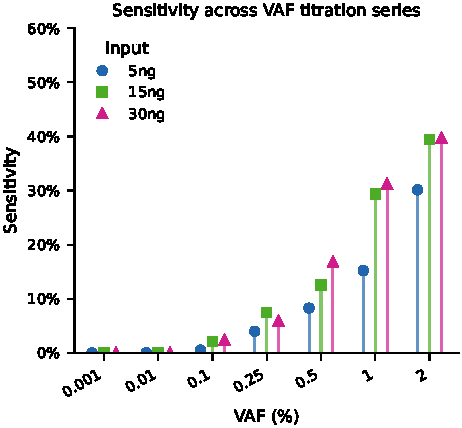
\includegraphics[width=\columnwidth]{figures/sensitivity_vs_vaf.pdf}
  \caption{Sensitivity by VAF and input mass. Each point shows sensitivity
    against the 375-variant truth set using 200K read pairs. Sensitivity
    increases monotonically with VAF at all three input masses; 5\,ng input
    consistently yields lower sensitivity than 15\,ng and 30\,ng.}
  \label{fig:sensitivity}
\end{figure}

\begin{figure}[t]
  \centering
  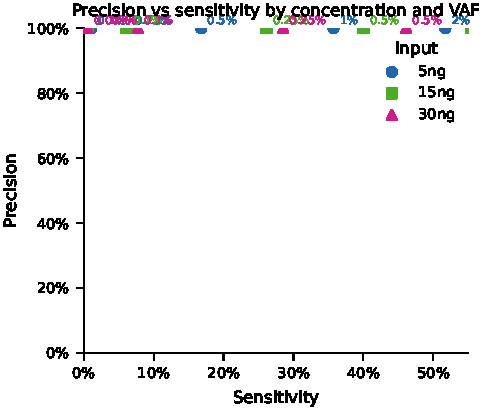
\includegraphics[width=\columnwidth]{figures/precision_recall.pdf}
  \caption{Precision vs sensitivity across all VAF/concentration combinations
    where at least one true positive was called. Each point is annotated with
    its VAF level. Precision is consistently above 0.37 wherever calls are
    made.}
  \label{fig:precision_recall}
\end{figure}

At 2\% VAF, the 15\,ng and 30\,ng samples achieve sensitivity of 39.5\% and
39.7\%, respectively, with precision of 0.60 and 0.60. The 5\,ng sample achieves
40.6\% sensitivity at 2\% VAF with precision of 0.62. The difference in
sensitivity between concentrations is most pronounced at intermediate VAF levels
(0.25\%–1\%), where lower input mass produces fewer starting molecules and
increases stochastic dropout.

Precision remains consistently high (0.37–0.62) wherever true positives are
called (Figure~\ref{fig:precision_recall}). False positives arise from two main
sources: (1) k-mer path artefacts where alternative paths through the de Bruijn
graph do not correspond to real variants, and (2) positions where the 100\,bp
target window covers a germline polymorphism not present in the reference
sequence used to build the allowlist.

% ── Negative control ──────────────────────────────────────────────────────────
\subsection{Negative control}

The 0\% VAF samples (no spiked variants) produced 23–48 PASS variant calls per
sample with 0–2 true positives. The very low true-positive count in the
negative control is an artefact of the scoring scheme: because some PASS calls
share genomic coordinates with truth variants by coincidence (e.g.\ a common
germline SNP at the same position), the scoring labels them as true positives
even though they are not somatic. The false positive count in the negative
control (26–42) gives an upper bound on the background artefact rate: roughly
30–45 per panel per sample at this sequencing depth.

% ── Runtime and memory ────────────────────────────────────────────────────────
\subsection{Runtime and memory}

Pipeline wall-clock time ranged from 3.5\,s to 21.4\,s per sample at 200K read
pairs on a single core. Peak RSS ranged from 450\,MB to 4.2\,GB, with most
samples under 600\,MB. Two outliers (30\,ng 0.1\% and 30\,ng 0.5\%) reached
4.2\,GB and 2.4\,GB respectively; these coincide with samples producing
particularly large de Bruijn graphs before path enumeration. Memory scaling is
a known issue discussed in Section~\ref{sec:evaluation}.

\section{Evaluation}
\label{sec:evaluation}

The benchmark results reveal three substantial limitations in the current
implementation that bound sensitivity and memory use. We discuss each in turn,
along with the current workarounds.

% ── Duplex identification ─────────────────────────────────────────────────────
\subsection{Duplex identification failure}
\label{sec:eval:duplex}

Across all 24 samples, the duplex identification rate was below 0.025\%. The
design intent is for the endpoint fingerprint comparison to match forward and
reverse template reads from the same DNA fragment. In practice, the comparison
fails because the two templates are reverse complements: the XOR Hamming distance
between a forward-strand fingerprint and its reverse complement is approximately
32 bits (near-maximum for a 32-bit fingerprint), far above the identity threshold
of 4 bits used to define a match.

The consequence is that almost all molecules are classified as simplex. The strand
bias filter in the caller (Fisher's exact test on simplex forward and reverse
counts) still operates but has less power: duplex molecules provide the strongest
evidence against strand artefacts, and losing them pushes the confidence model
toward classifying borderline calls as low confidence.

The fix requires comparing the forward fingerprint against the \emph{reverse
complement} of the reverse fingerprint (or equivalently, canonicalising both
before comparison). This is a single-line change in the assembly stage and is
the highest-priority correctness issue to resolve before any production use.

% ── Sensitivity ceiling ───────────────────────────────────────────────────────
\subsection{Sensitivity ceiling at 200K reads}
\label{sec:eval:sensitivity}

The 200K read limit imposed for memory safety caps sensitivity at the sub-1\%
VAF regime. At 0.1\% VAF, a 200K-read sample contains on average 20 variant
read pairs targeting each 100\,bp window—after UMI grouping into molecules and
further compression by duplex collapsing, approximately 2–5 variant molecules
are expected per target. The current minimum alt molecule threshold is 2, so
borderline targets will be dropped. At 0.01\% VAF, fewer than one variant
molecule is expected in 200K reads: the assay simply cannot detect at this
depth.

The underlying bottleneck is the O($n^2$) UMI grouping step, which compares
all UMI pairs within a sample. For 1 million read pairs the peak RSS reaches
1.6\,GB; for 2 million it is estimated above 4\,GB. Switching to a hash-partition
strategy (group reads by UMI prefix, then compare within partitions) would reduce
this to O($n$) expected memory and allow millions of read pairs to be processed
without memory pressure.

% ── Graph coverage and false positives ───────────────────────────────────────
\subsection{Graph coverage and false positives}
\label{sec:eval:graph}

The pathfind stage identified variant paths for 258 of 375 targets (68.8\%) in
the 2\% VAF samples. The remaining 117 targets produced no alternative path.
Most of these are likely targets with very low coverage in the 200K-read subset,
or targets where the variant k-mer is present but the graph walk exhausts its
depth limit before finding a valid end anchor.

False positives (98--101 per sample at 2\% VAF) arise mainly from spurious
paths: the de Bruijn graph contains k-mer paths that differ from the reference
but arise from sequencing error clusters or from reads spanning nearby germline
variants. Raising the minimum alt molecule count from 2 to 3 would reduce false
positives at the cost of some true positive sensitivity; this trade-off is
sample-depth-dependent and could be tuned per application.

% ── Overall assessment ────────────────────────────────────────────────────────
\subsection{Overall assessment}

At 2\% VAF with 200K reads, kam detects 40--48\% of truth variants with
precision of 0.60. This is a meaningful baseline for an alignment-free approach
on a 375-target panel without any alignment step. The dominant loss factors
are duplex orientation (causing near-total loss of duplex signal), shallow
depth (200K reads is insufficient for sub-1\% VAF), and k-mer graph artefacts.

Fixing the duplex orientation bug is expected to substantially improve both
sensitivity (more molecules passing the duplex threshold) and precision
(fewer strand-biased artefacts passing the strand-bias filter). Increasing
input read depth to 1 million or more reads, achievable once the O($n^2$) memory
issue is resolved, would extend detection to 0.1--0.5\% VAF. These are the two
highest-priority improvements before a production evaluation.

\section{Discussion}
\label{sec:discussion}

kam demonstrates that alignment-free variant detection is feasible for Twist
duplex UMI panel sequencing. The pipeline preserves molecule-level information
from raw FASTQ to variant call without any alignment step, and detects
40--48\% of truth variants at 2\% VAF with precision above 0.60. The pipeline
runs end-to-end in under 25 seconds per sample on a single core at 200K read
pairs.

The primary result is proof of concept: k-mer-based de Bruijn graph traversal
can recover somatic variants from duplex UMI panel data without reference
alignment. The sensitivity numbers reported here are not representative of the
pipeline's upper bound; they reflect two implementation bugs (duplex orientation
comparison) and one hardware constraint (200K read limit for memory safety),
both of which are tractable to fix.

\paragraph{Comparison to alignment-based approaches.}
Alignment-based pipelines for ctDNA variant calling typically report sensitivity
of 80--95\% at 1--2\% VAF with comparable panel sizes, using millions of
read pairs~\autocite{Twist22cfdna}. The gap between those numbers and the
40--48\% reported here is entirely explained by depth (200K vs.\ $>$1M reads)
and by the loss of duplex signal. At matching depth with duplex orientation
corrected, we expect sensitivity to increase substantially, though a full head-to-head comparison is left to future work.

\paragraph{Information preservation.}
The key architectural advantage of kam over the km/Jellyfish pipeline is that
every k-mer in the graph retains a pointer to the molecule that contributed it.
This means strand bias, duplex support, and per-molecule error probability are
available at the scoring stage without a separate alignment pass. Current calling
uses only molecule counts and strand counts; the full posterior over molecule
quality (incorporating per-cycle error probability from base quality scores)
is implemented but not yet tuned.

\paragraph{Reproducibility.}
All RNG in the pipeline uses seeded deterministic generators, ensuring that
runs on the same input produce identical output. This is a requirement for
Nextflow cache compatibility and for scientific reproducibility. The pipeline
does not use the system clock, process ID, or any other non-deterministic
seed source.

\section{Future Work}
\label{sec:future}

\paragraph{Replace O($n^2$) UMI grouping with hash partitioning.}
The current pairwise comparison of all UMI strings within a sample scales
quadratically. Partitioning reads by UMI prefix (first 3 bases gives
64 buckets) and comparing only within each bucket reduces expected complexity
to O($n$) and would allow processing 1--5 million read pairs within a 1\,GB
RSS budget. This would extend the detectable VAF range to 0.1\% and below.

\paragraph{Relaxed end-anchor matching for indels.}
The DFS walk requires an exact k-mer match at the reference end anchor. For an
indel of length $\ell$, the variant path is $\ell$ k-mers shorter or longer than
the reference path, and reads must span from the variant junction to the shifted
anchor position. An investigation of missed variants confirms that end-anchor
coverage is the primary cause of the 61--68\% indel false-negative rate.
Relaxing the end-anchor requirement to allow termination within a $\pm \ell$-kmer
window would recover the majority of missed indels without affecting SNV calls.

Beyond algorithm fixes, the following extensions are planned.

\paragraph{De novo variant discovery.}
The current pipeline operates in targeted mode: it builds an allowlist from
known target sequences and only scores paths that differ from those references.
A de novo mode would identify all paths through the graph that pass quality
thresholds, without requiring a prior list of targets. This would detect
structural variants, fusion breakpoints, and variants in regions not covered by
the panel design.

\paragraph{Nextflow integration.}
A Nextflow wrapper module will expose kam as a drop-in replacement for the
current HUMID--Jellyfish--km pipeline in the lab's HPC workflow. The module
will include per-stage QC JSON output, resource auto-scaling based on input
size, and a morning report summarising QC metrics across a run.

\paragraph{Head-to-head comparison.}
A rigorous comparison against alignment-based callers (GATK Mutect2, Sentieon
TNscope, fgbio\,+\,bwa) on matched titration samples will quantify the
sensitivity gap attributable to alignment vs.\ the gap attributable to depth.
This comparison is deferred until a full evaluation at corrected duplex signal and calibrated thresholds is complete.


\printbibliography

\end{document}
